% A '%' character causes TeX to ignore all remaining text on the line,
% and is used for comments like this one.

\documentclass{article}      % Specifies the document class
\usepackage{amsmath, nccmath}
\usepackage{enumitem}
\usepackage{graphicx}
\usepackage[utf8]{inputenc}
\usepackage{listings}
\usepackage{xcolor}
\graphicspath{ {./} }
\definecolor{codegreen}{rgb}{0,0.6,0}
\definecolor{codegray}{rgb}{0.5,0.5,0.5}
\definecolor{codepurple}{rgb}{0.58,0,0.82}
\definecolor{backcolour}{rgb}{0.95,0.95,0.92}

\lstdefinestyle{mystyle}{
    backgroundcolor=\color{backcolour},   
    commentstyle=\color{codegreen},
    keywordstyle=\color{magenta},
    numberstyle=\tiny\color{codegray},
    stringstyle=\color{codepurple},
    basicstyle=\ttfamily\footnotesize,
    breakatwhitespace=false,         
    breaklines=true,                 
    captionpos=b,                    
    keepspaces=true,                 
    numbers=left,                    
    numbersep=5pt,                  
    showspaces=false,                
    showstringspaces=false,
    showtabs=false,                  
    tabsize=2
}

\lstset{style=mystyle}

\title{CEE 498 Applied Machine Learning - HW4}  % Declares the document's title.
\author{Rini Jasmine Gladstone (rjg7) and Maksymillian Podraza(podraza3)}      % Declares the author's name.
\date{March 30, 2020}      % Deleting this command produces today's date.

\newcommand{\ip}[2]{(#1, #2)}
                             % Defines \ip{arg1}{arg2} to mean
                             % (arg1, arg2).

%\newcommand{\ip}[2]{\langle #1 | #2\rangle}
                             % This is an alternative definition of
                             % \ip that is commented out.

\begin{document}             % End of preamble and beginning of text.

\maketitle                   % Produces the title.


\section{Problem 1}      % Produces section heading.  Lower-level
                             % sections are begun with similar 
                             % \subsection and \subsubsection commands.

\subsection{Part a}

We followed the following steps for this part.

\begin{enumerate}[label=(\alph*)]
\item Built a function for creating 10 x 10 patches and extracting these patches from a 4x4 grid of an image

\begin{lstlisting}
#Creating 4x4 grid of 10x10 patches
def patch_creation(image):
    patches = []
    x=[0,6,12,18]
    y=[0,6,12,18]
    for i in x:
        for j in y:
            patch = image[i:i+10,j:j+10].reshape(-1,100)
            patches.append(patch)
    return(patches)
\end{lstlisting}

\item Created patches for all 60,000 training images. 

\begin{lstlisting}
#reshaping each 784 1-d array into 28x28 2-d array and creating patches for each image
training_patches=[]
for i in range(60000):
    image = train_set[0][i].reshape(28,28)
    training_patches.append(patch_creation(image))
\end{lstlisting}

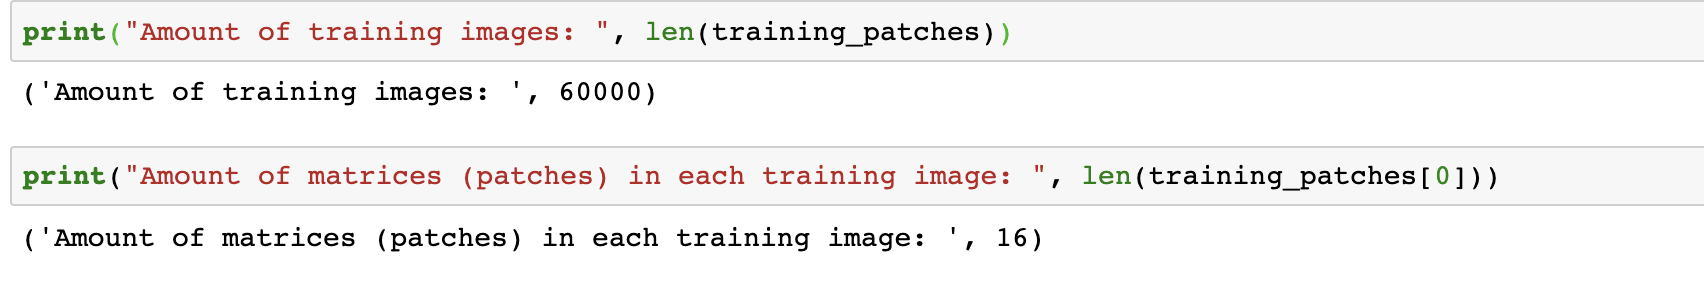
\includegraphics[width=\textwidth]{trainingimages}

An example of the train image with the patches is as shown below.

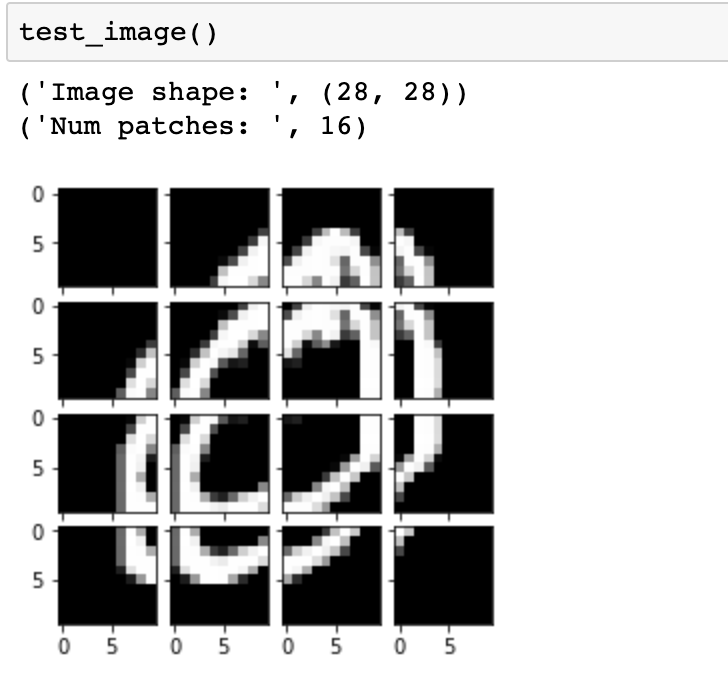
\includegraphics[width=\textwidth]{testimage}

\item For each training image,  one of these patches is chosen uniformly and at random. This dataset of 60,000 patches is sub-sampled uniformly and at random to produce a 6000 element dataset

\begin{lstlisting}
#Choosing 1 patch from the 16 previously created for each image at random and appending to training list
train_cluster=[]
for i in range(60000):
    n = random.randint(0, 15)
    train_cluster.append(training_patches[i][n])
#creates a list of 6000 numbers where each is between 0 - 59999
indices = random.sample(range(60000), 6000)
#appending randomly sampled patches using the previously created list of indices
train_cluster_sample=[]
for ind in indices:
    train_cluster_sample.append(train_cluster[ind])
\end{lstlisting}

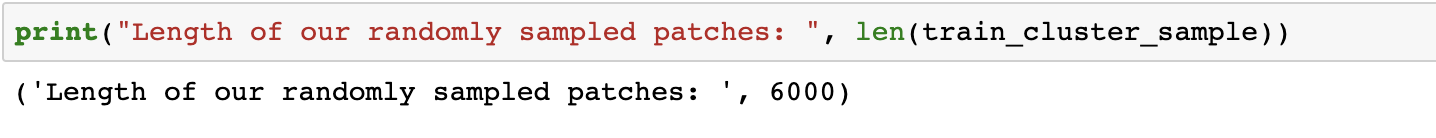
\includegraphics[width=\textwidth]{lengthpatch}

\item The above dataset is clustered to 50 centres. 

\begin{lstlisting}
#creating a 6000x100 matrix of zeros that where each row will be one of our samples
training_matrix = np.zeros((6000,100))
for i in range(6000):
    #making eacch row a random patch
    training_matrix[i,:] = train_cluster_sample[i][0]
# create kmeans object
kmeans = KMeans(n_clusters=50)
# fit kmeans object to data
kmeans.fit(training_matrix)
# save new clusters for chart
y_km = kmeans.predict(training_matrix)
\end{lstlisting}

\item Assigned the closest cluster to all the patches of the 60,000 training images.

\begin{lstlisting}
training_matrix_60k = np.zeros((60000,100))
for i in range(60000):
    training_matrix_60k[i,:] = train_cluster[i][0]
y_km_60k = kmeans.predict(training_matrix_60k)
\end{lstlisting}

\item Subset datasets for each cluster centre and cluster them again to 50 clusters.

\begin{lstlisting}
cluster_dict = {}
for i in range(50):
    key = str(i)
    subtrain_matrix = training_matrix_60k[y_km_60k==i,:]
    kmeans_sub = KMeans(n_clusters=50)
    kmeans_sub.fit(subtrain_matrix)
    cluster_dict[key] = kmeans_sub 
    y_km_sub = kmeans_sub.predict(subtrain_matrix)
\end{lstlisting}

\end{enumerate}

\subsection{Part b}

We followed the following steps for this part.

\begin{enumerate}[label=(\alph*)]
\item Built a function for padding the images

\begin{lstlisting}
def pad_with(vector, pad_width, iaxis, kwargs):
    pad_value = kwargs.get('padder', 0)
    vector[:pad_width[0]] = pad_value
    vector[-pad_width[1]:] = pad_value
\end{lstlisting}

\item Built a function for creating 9 sub-patches for each of the 10x10 patch in the 4x4 grid.
\begin{lstlisting}
def patch_b(image):
    patches16 = []
    x_ = [0, 1, 2]
    y_ = [0, 1, 2]
    x=[0,6,12,18]
    y=[0,6,12,18]
    for i in x:
        for j in y:
            patches9 = []
            for k in x_:
                for l in y_:
                    patch = image[i+k:i+k+10, j+l:j+l+10].reshape(-1,100)
                    patches9.append(patch)
            patches16.append(patches9)
    return patches16
\end{lstlisting}

\item The sub patches were created for 10,000 testing images and 6,000 training images.

\begin{lstlisting}
testing_patches = []
testing_labels = []
for i in range(10000):
    testing_reshaped = test_set[0][i].reshape(28,28)
    testing_labels.append(test_set[1][i])
    testing_padded = np.pad(testing_reshaped, 1, pad_with)
    testing_patched = patch_b(testing_padded)
    testing_patches.append(testing_patched)
\end{lstlisting}

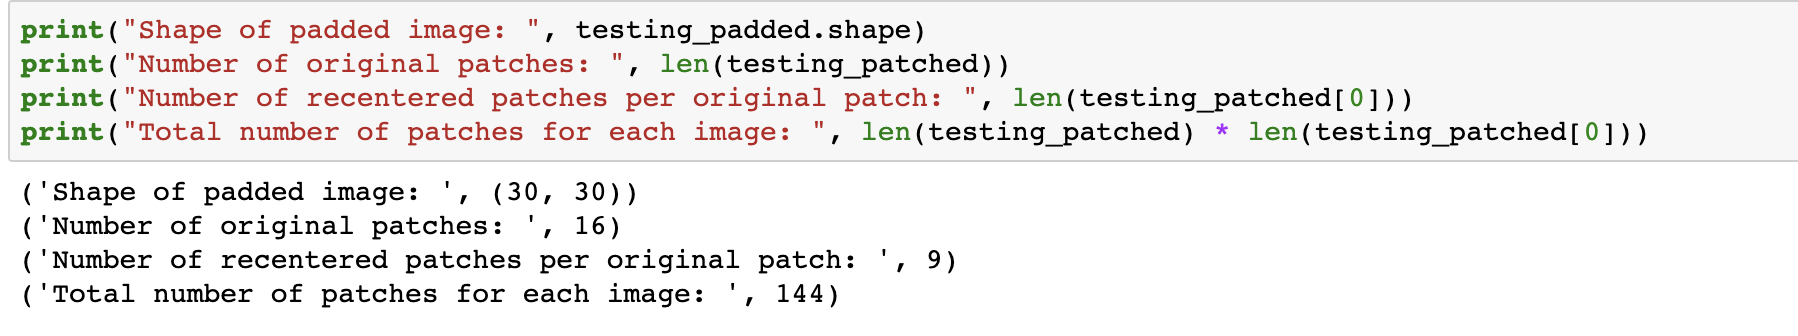
\includegraphics[width=\textwidth]{testpad}

\begin{lstlisting}
training_patches = []
random_indices = random.sample(range(60000), 6000)
training_labels = []
for i in random_indices:
    training_reshaped = train_set[0][i].reshape(28,28)
    training_labels.append(train_set[1][i])
    training_padded = np.pad(training_reshaped, 1, pad_with)
    training_patched = patch_b(training_padded)
    training_patches.append(training_patched)
\end{lstlisting}

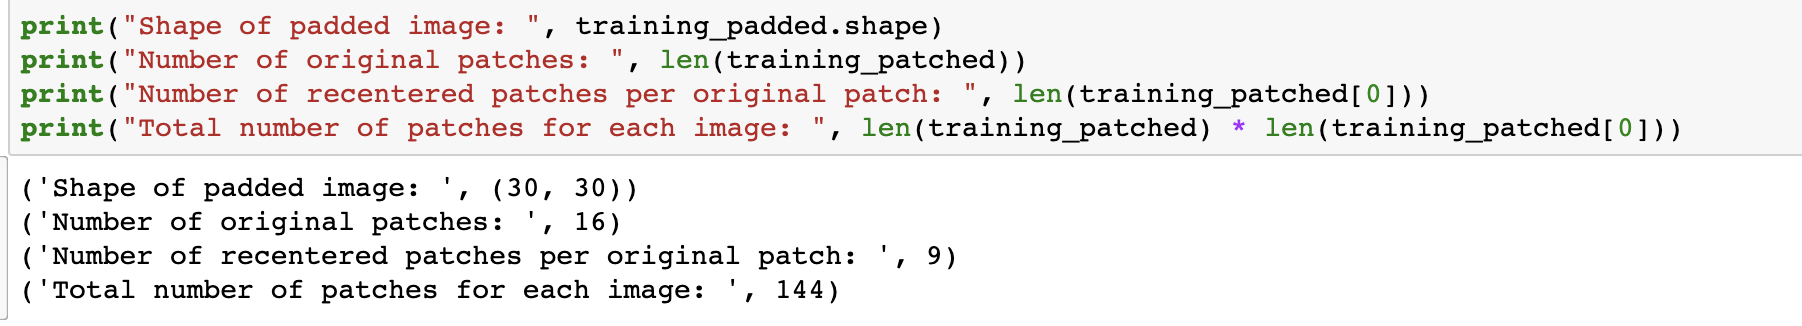
\includegraphics[width=\textwidth]{trainpad}

\item Then, we built a function for finding the cluster and sub cluster for each of the sub patches.

\begin{lstlisting}
def finding_cluster(data,num_images=10000,num_grids=16,num_patches=9):
    data_matrix_long = np.zeros((num_images*num_grids*num_patches,100))
    z=0
    for i in range(num_images):
        for j in range(num_grids):
            for k in range(num_patches):
                data_matrix_long[z,:] = data[i][j][k]
                z=z+1
    #Finding the main 50 clusters
    data_km_long = kmeans.predict(data_matrix_long)
    data_50clusters= np.zeros((num_images,num_grids,num_patches))
    z=0
    for i in range(num_images):
        for j in range(num_grids):
            for k in range(num_patches):
                data_50clusters[i,j,k] = data_km_long[z]
                z=z+1
    data_2500clusters= [[['000_000' for i in range(num_patches)] for j in range(num_grids)] for k in range(num_images)]
    subcluster_data_fit = np.zeros((1,100))
    z=1
    #Finding the subclusters of each patch
    for i in range(num_images):
        for j in range(num_grids):
            for k in range(num_patches):
                cluster = data_50clusters[i,j,k]
                subcluster_data_fit[0,:] = data[i][j][k]
                fitted_centre=cluster_dict[str(int(cluster))].predict(subcluster_data_fit)
                text=str(int(cluster))+'_'+str(fitted_centre[0])
                data_2500clusters[i][j][k]= text
                if z%10000==0 and z>=10000:
                    print(str(z*100/(num_images*num_grids*num_patches))+'% done')
                z=z+1
    return(data_2500clusters)
\end{lstlisting}

\item We built a function for creating the histogram, i.e. we built the dataset of shape 10,000 x 2,500 for testing and 6,000 x 2,500 for training with each column giving the number of patches with a certain cluster\_subcluster.

\begin{lstlisting}
def histogram_patch_creation(data,num_images=10000,num_grids=16,num_patches=9):
    colnames=['image_num']
    for i in range(50):
        for j in range(50):
            colnames.append(str(i)+'_'+str(j))
    df=np.zeros((num_images,2501))
    hist_patches = pd.DataFrame(df,columns = colnames)
    hist_patches['image_num']=range(num_images)
    z=1
    for i in range(num_images):
        for j in range(16):
            for k in range(9):
                hist_patches.loc[i,data[i][j][k]]+=1
                if z%10000==0 and z>=10000:
                    print(str(z*100/(num_images*num_grids*num_patches))+'% done')
                z=z+1
    return(hist_patches)
\end{lstlisting}

\begin{lstlisting}
#Creating testing data of shape 10000x2500
test_hist_patches=histogram_patch_creation(test_2500clusters,10000,16,9)
#Creating training data of shape 6000x2500
train_2500clusters = finding_cluster(training_patches, 6000, 16, 9)
train_hist_patches=histogram_patch_creation(train_2500clusters,6000,16,9)
\end{lstlisting}
\end{enumerate}

\subsection{Part c}

We built a random forest classifier using the training data created as above and tested it on the testing data. Number of trees is set to be 100 and there is no depth set.

\begin{lstlisting}
from sklearn.ensemble import RandomForestClassifier
from sklearn.metrics import accuracy_score
from sklearn.metrics import confusion_matrix
rf = RandomForestClassifier(n_estimators=100, oob_score=True).fit(train_hist_patches,training_labels)
test_y_pred = rf.predict(test_hist_patches)
train_y_pred = rf.predict(train_hist_patches)
\end{lstlisting}

\begin{lstlisting}
#Accuarcy on the training dataset
accuracy_score(training_labels,train_y_pred)*100
\end{lstlisting}

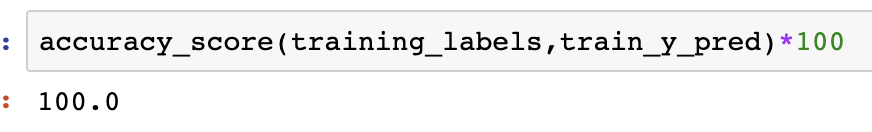
\includegraphics[width=\textwidth]{trainaccuracy}

\begin{lstlisting}
#Accuarcy on the testing dataset
accuracy_score(testing_labels,test_y_pred)*100
\end{lstlisting}

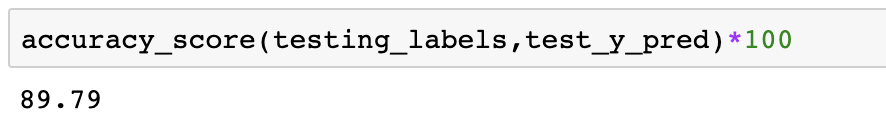
\includegraphics[width=\textwidth]{testaccuracy}


\subsection{Part d}

\subsection{Part e}






%\section{Appendix}

%The code for Part 1.a is given below. 
%\lstinputlisting[language=R]{Qn1.R}



\end{document}